
%----------------------------------------------------------------------------------------
%	PACKAGES AND DOCUMENT CONFIGURATIONS BY DANIEL HEDIGER
%----------------------------------------------------------------------------------------

\documentclass{article}

\usepackage[version=3]{mhchem} % Package for chemical equation typesetting
\usepackage{siunitx} % Provides the \SI{}{} and \si{} command for typesetting SI units
\usepackage{graphicx} % Required for the inclusion of images
\usepackage{natbib} % Required to change bibliography style to APA
\usepackage{amsmath} % Required for some math elements 
\usepackage{german}
\usepackage{float}
\restylefloat{figure}
\usepackage[utf8]{inputenc}
\setlength\parindent{0pt} % Removes all indentation from paragraphs
\renewcommand{\labelenumi}{\alph{enumi}.} % Make numbering in the enumerate environment by letter rather than number (e.g. section 6)
\usepackage{blindtext}

%\usepackage{times} % Uncomment to use the Times New Roman font

%----------------------------------------------------------------------------------------
%	DOCUMENT INFORMATION
%----------------------------------------------------------------------------------------

\title{Physiklabor \\ Laborbericht \\ Optik} % Title

\author{Daniel \textsc{Hediger} \\ Lucien \textsc{Egloff}} % Author name



\date{\today} % Date for the report

\begin{document}

\maketitle % Insert the title, author and date

\begin{center}
\begin{tabular}{l r}
	Ausführungsdatum: & Dezember 7, 2016 \\ % Date the experiment was performed
	Dozent: & Dr.Ackermann \\% Instructor/supervisor
	Version: & 1.0
	
\end{tabular}
\end{center}
\begin{figure}[H]
	\centering
	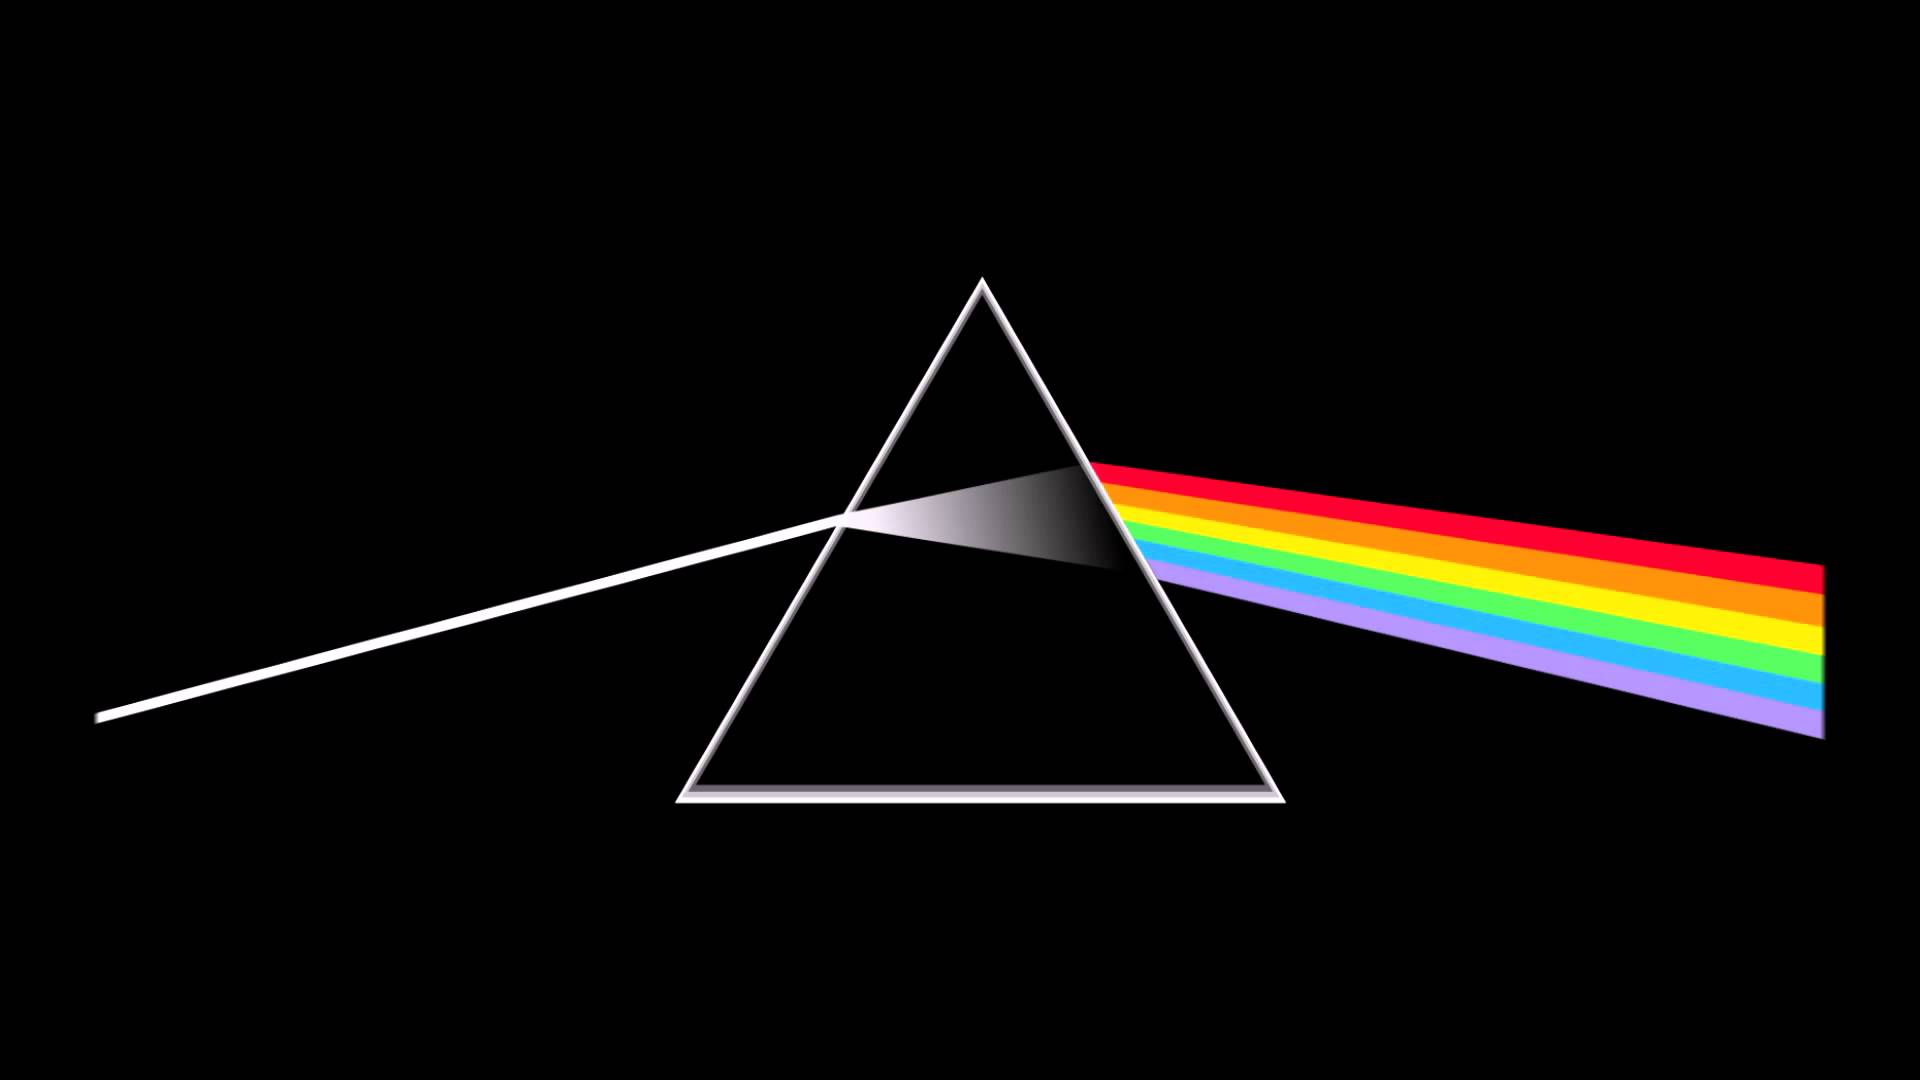
\includegraphics[scale=0.2]{dsotm.jpg} 
\end{figure}
\newpage
\tableofcontents 

%----------------------------------------------------------------------------------------
%	SECTION 1
%----------------------------------------------------------------------------------------
\newpage
\section{Versuch 1 Haardurchmesser}
\subsection{Versuch}
Es wurde mit einem grünen Laserstrahls auf ein Haar gehalten. Die Beugung der Lichtwellen konnte
man an der Wand im Hintergrund mit drei Maxima erkennen. Indem die Abstände der Maxima und
der Abstand der Wand gemessen wurde, konnte die Dickes des Haars berechnet werden. Der Versuch
wurde ebenfalls mit einer Kohlenfaser durchgeführt. Der Laserstrahl muss breiter sein als das
Objekt.
\subsection{Messwerte}

\textbf{Haar:}

\begin{tabular}{l r}
	Abstand des Maxima dk & \textbf{45mm}\\
	k	&\textbf{1}\\
	Abstand zu Wand L&\textbf{3000mm} \\
	Wellenlänge Lasers $\lambda$ & \textbf{532nm}
\end{tabular}

\textbf{Kohlefaser:}

\begin{tabular}{l r}
	Abstand des Maxima dk & \textbf{150mm}\\
	k	&\textbf{1}\\
	Abstand zu Wand L&\textbf{3000mm}\\
	Wellenlänge Lasers $\lambda$ & \textbf{532nm}
\end{tabular}

\subsection{Berechnungen}
\textbf{Haar}
\begin{equation}
\varphi = arctan(\frac{dk}{L}) = \frac{45}{3000}
\end{equation}
\begin{equation}
L = y \cdot \frac{k+0.5}{sin(\varphi)}= \underline{\underline{text}} 
\end{equation}
\textbf{Kohlefaser}
\begin{equation}
\varphi = arctan(\frac{dk}{L}) = \frac{45}{3000}
\end{equation}
\begin{equation}
L = y \cdot \frac{k+0.5}{sin(\varphi)}= \underline{\underline{text}} 
\end{equation}
\subsection{Fehlabschätzung}
\begin{tabular}{l r}
	Haardicke mit dem Mikrometer gemessen & \textbf{0.045mm}\\
	Kohlefaser mit dem Mikrometer gemessen	&\textbf{0.005}\\
\end{tabular}
Das Haar konnte ziemlich genau gemessen werden, bei der Kohlefaser kann es sein, dass ein Bündel
von Kohlefaser gemessen wurde, das es schwer war diese voneinander zu trennen.
\section{Versuch 2 Spurabstand CD/DVD}
\subsection{Versuch}
Der Spurabstand wurde durch die Reflektion des Laserstrahls und dessen Beugung ähnlich wie im
Haardurchmesser-Versuch ermittelt. Der grüne Laserstrahl trifft auf die Oberfläche der CD, dringt
durch die Gitterstruktur und Reflektiert an der Rückseite der CD. Die reflektierten Maxima konnten auf
eine Oberfläche in der Nähe des Lasergerätes projiziert werden. Es wurde wiederum der Winkel ermittelt,
und mit der Wellenlänge des Lasers der Spurabstand gerechnet. Weil es sich um eine Gitterstruktur
handelt muss beim Rechnen nicht 0.5 zum k addiert werden.
\subsection{title}

\end{document}